\section{Other tools}
There are a lot of different bibliography management tools out there.
To uncover potential features already in existence we'll try to
uncover what those tools are and what features they provide.

\subsection{Mendeley}
Mendeley is mainly a tool for bibliography management, of it's main
features it can extract bibliography information from PDF-files, and a
heavy integration with DOI lookups, to gather and update information
from a central database.  Like BibTeX, it does not facilitate any
systems for detecting inconsistencies such as spelling errors,
revision numbers or initials.  Mendeley does not have any plugin/add
on system, so it's unlikely that there is any third party tools to
remedy this \cite{mendeley_features}.

A search through Mendeley's request database reveals the same as the
testing and features page.  There is a lot of requests for features
such as spell checking, fixing capitalization inconsistencies and bulk
DOI lookups \cite{mendeley_request_spellcheck,
  mendeley_request_lowercase,
  mendeley_request_capitalization, mendeley_request_bulk_doi}.

\subsection{EndNote and RefMan}
EndNote is another tool for reference mangement, from Thompson
Reuters.  When inspecting the feature set of EndNote it seems that it
provides tools for detecting abbreviations in journals and ways to
standardize those \cite{endnote_basic_features, endnote_x7_features}.
The tools however is only used to format the names when exported or
used as references, mapping from a predefined set of know
abbreviations, the tool does not fix the naming issues internally in
the files\cite{endnote_terms_journals}.  Remedying this by using DOI
lookups also seems to create duplicate entries rather than updating
the current making the issues even worse. \remark{Own testing}

RefMan is another tool provided by Thompson Reuters, on the homepage
they recommend you to switch to EndNote \cite{refman_switch}.
Inspecting the features it does not seem to offer anything of
relevance that EndNote does not \cite{refman_features}, so it has not
been evaluated further.

\subsection{RefWorks}
The approach from RefWorks is a web based platform.  Compared to the
other tools the features is very limited and there is close to no
detection of errors.  Two things to note though is that is contrary to
the other tools actually specify how you are supposed to fill the
fields where you fill them and it actually tries to detect if the
author name is malformed, although it only seems to detect if you type
``John Doe'' rather than ``Doe, John'' as it expects, as can be seen
at figure-\ref{fig:refworks-detect-formatting}.

\begin{figure}[h]
    \centering
    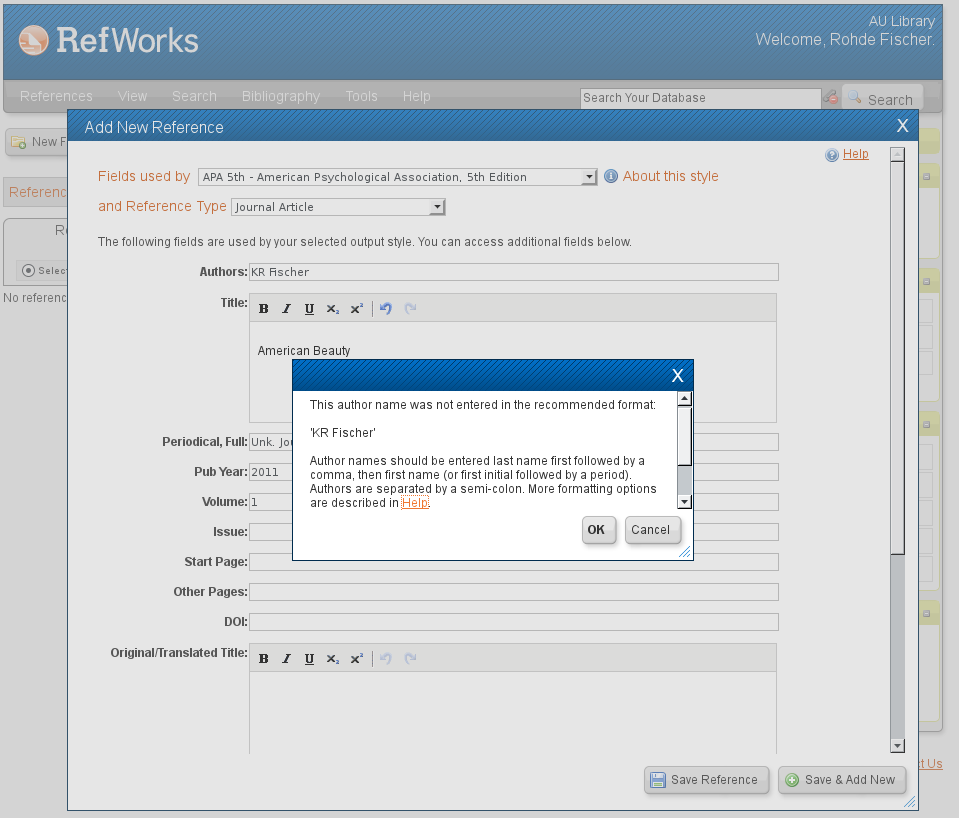
\includegraphics[width=0.8\textwidth]{refworks-detect-formatting}
    \caption{RefWorks detects some formatting on the name field}
    \label{fig:refworks-detect-formatting}
\end{figure}

The fact that RefWorks does not do much more is in part remedied by
most modern browsers, because they tend to include spell checkers for
the input fields.

\subsection{Zotero}
Zotero has a built in spell checker for notes, however the spell
checker is not applied for things like titles, which prevents it from
detecting those errors.  Also it does not seem that it does anything
to detect abbreviations.  Unfortunately Zotero does not have a list of
features directly, apart from some very superficial texts on the front
page \cite{zotero_features}.

Unlike the other systems Zotero has a plugin system, which makes it
possible that a user created plugin for these features exists, however
none was found using the official list of plugins
\cite{zotero_plugins} nor by a normal search engine.

There is a limited mechanism for detecting abbreviations in Zotero, in
its jar-file there is a list of known abbreviations which it can use
to chose the correct abbreviation when exporting, entering a known
abbreviation does not seem to correct it to the non-abbreviated
version.  This list can be manually edited, and overruled
\cite{zotero_abbreviations}

\subsection{Others?}
\remark{Mostly notes to myself}

http://jabref.sourceforge.net/resources.php

%%% Local Variables:
%%% mode: latex
%%% TeX-master: "thesis"
%%% End:
